\documentclass{css}
%\documentclass[english]{css}

\usepackage[dvipdfmx]{graphicx}
\usepackage{latexsym}
\usepackage{listings}
\usepackage{url}
\urlstyle{same}
\usepackage{tikz}
\usetikzlibrary{arrows.meta}

\newcommand{\cssyear}[0]{2026}
\newcommand{\cssname}[0]{CSS 2026}
\newcommand{\cssversion}[0]{2026/06/01}
\newcommand{\cssemail}[0]{css2026-office@iwsec.org}

\makeatletter
\newcommand\newblock{\hskip .11em\@plus.33em\@minus.07em}
\makeatother

\begin{document}

%% 本文が和文の場合，タイトル・著者名・著者所属・概要は，和文・英文共に必須．

\title{脆弱性情報の上流は安定していない: \\ 公開前検査による116日間の全数観測}
\etitle{Vulnerability Feeds Are Not Stable: A 116-Day Exhaustive Observation via Pre-Publication Inspection}

\affiliate{FUTURE}{フューチャー株式会社\\
Future Corporation}

\author{篠原 俊一}{Shunichi Shinohara}{FUTURE}[s.shinohara.yx@future.co.jp]
\author{中岡 典弘}{Norihiro Nakaoka}{FUTURE}[n.nakaoka.46@future.co.jp]
\author{神戸 康多}{Kota Kanbe}{FUTURE}[k.kanbe.r4@future.co.jp]

\begin{abstract}
脆弱性データベースは多数の上流データソースを集約して構築されるが，上流は必ずしも安定せず，データの消失や公開済みアドバイザリの遡及的な書き換えが現実に起きている．
本研究では，この不安定性を定量観測するため，OSS脆弱性スキャナVulsのDB公開CIに公開前検査を実装した．
検査は公開候補と直前の公開版を，検知結果と検知条件構造の2観点で比較し，変動率が閾値を超えた場合は公開を保留して人間の確認に委ねる．
116日間の本番運用の全数調査では69件のイベントで検査が発動し，全工程を履歴管理する既報の基盤を用いて，その全てについて原因を上流データの変化か，変換やDB構築や取得設定といった自前の処理かのいずれかに帰属できた．
日常変動と構造的イベントは変動率で桁が分離しており，閾値による単純な判定が実用になること，また欠損DBの公開を2回，異常な候補DBの公開を1回阻止したことを示す．
\end{abstract}

\begin{jkeyword}
脆弱性データベース，データ品質，公開前検査，履歴管理，ソフトウェアサプライチェーン
\end{jkeyword}

\begin{eabstract}
Vulnerability databases are built by aggregating many upstream data sources, but these upstreams are not always stable: data disappears, and published advisories are retroactively rewritten.
To quantify this instability, we implemented a pre-publication inspection in the CI pipeline that builds and publishes the database of Vuls, an open-source vulnerability scanner.
The inspection compares each publication candidate with the previously published version in terms of detection results and detection-criteria structure, and when the change rate exceeds a threshold, it withholds publication pending human review.
In an exhaustive study covering 116 days of production operation, the inspection was triggered by 69 events, and our previously reported infrastructure, which keeps every pipeline stage under version control, allowed us to attribute every event to either upstream data changes or our own processing such as data transformation, database construction and fetch configuration.
We show that everyday fluctuation and structural events are separated by an order of magnitude in change rate, making this simple threshold-based inspection practical, and that the inspection blocked the publication of databases with missing data twice and of an anomalous candidate once.
\end{eabstract}

\begin{ekeyword}
Vulnerability Database, Data Quality, Pre-Publication Inspection, History Management, Software Supply Chain
\end{ekeyword}

\maketitle

\section{はじめに}
\label{sec:intro}

脆弱性対応の実務は，ディストリビュータやベンダが公開するアドバイザリや脆弱性フィードを「正」として組み立てられている．
脆弱性スキャナはこれらを集約した脆弱性データベース(以下，脆弱性DB)に依存し，検知結果はフィードの内容をほぼそのまま反映する．
ここには，上流フィードは概ね安定しており，変化は新規脆弱性の追加という単調な形をとる，という暗黙の仮定が置かれている．
この仮定はどの程度正しいのだろうか．

我々はOSS脆弱性スキャナVuls\cite{vuls}のエコシステムにおいて，40超のデータソースから脆弱性DB(vuls.db)をCIで自動ビルドし，6時間おきに公開している．
前稿\cite{nakaoka2025}では，この収集(fetch)，変換(extract)，構築(db build)の全工程をバージョン管理システムと連携させ，脆弱性情報の変更履歴を客観的事実として追跡・再現可能にする履歴管理基盤を報告した．
本稿はその続編にあたる．
前稿の基盤が「脆弱性情報の変化を\textbf{記録できる}」ことを示したのに対し，本稿はその記録能力を使って「上流は実際に\textbf{どう変化しているか}」を系統的に測定し，さらにその測定をDBの公開品質管理として実用化した結果を報告する．

測定の装置は単純である．
公開直前の候補DBを，現に公開されている直前版(baseline)と自動比較し，変動率が閾値を超えたら公開を保留して人間に見せる．
我々はこれを\textbf{公開前検査}(diff guard)と呼ぶ．
導入の直接の動機は，自らのパイプライン変更と上流の破損データの複合，およびDBとスキャナのバージョン非互換によって「壊れたDB」を公開してしまった2件のインシデント(\ref{sec:incidents}節)であり，検査は第一義には安全ネットである．
しかし116日間の本番運用で得られた発動記録の全数調査は，副産物として，脆弱性情報の上流がいかに大きく，頻繁に，時に黙って動くかの縦断観測データとなった．

本稿の貢献は次の3点である．

\begin{enumerate}
\item \textbf{上流不安定性の実測}(\ref{sec:results}節，\ref{sec:discussion}節):
116日間・943 runの全数調査から69件の発動episodeを抽出し，59件を上流由来，10件を自前の処理由来に帰属した上で，上流の不安定性を分類・定量化した．
観測されたイベントは，可用性の不安定(月次データの消失とフラッピング)，完全性の危うさ(遡及的な再キュレーションやアナウンスのないサーバ側再編)，スケールの分布(日常変動と構造的イベントの桁分離)の3群に整理できる．
これらの上流の多くは他の脆弱性ツール(Trivy，Grype，OSV系等)も共有しており，知見はエコシステム横断で再利用可能である．
\item \textbf{原因帰属の方法論}(\ref{sec:method}節):
発動の原因をビルダ，抽出器，取得設定，上流の順に容疑を除外して確定する切り分け手順を定義し，全イベントに適用した．
各ステップは履歴管理基盤\cite{nakaoka2025}の対応する工程の履歴(DBメタデータ，抽出器のコミット履歴，rawデータのGit差分)に依拠しており，全工程の履歴管理が帰属の成立条件であることを示す．
\item \textbf{公開前検査の設計と運用機構}(\ref{sec:design}節):
検知結果差分とDB構造差分の2観点による検査本体に加え，監査証跡付き手動override(promote)，対象別閾値の統計的導出と定期的な再導出(grooming)という，検査を運用し続けるための機構を設計・実装した．
検査は欠損または異常な候補DBの公開を3回阻止した．
\end{enumerate}

\begin{figure}[tb]
\centering
\begin{tikzpicture}[font=\footnotesize, >=Stealth,
  b/.style={draw, rounded corners=1pt, align=center, inner sep=3pt, minimum height=5mm},
  hist/.style={b, fill=gray!15},
  lbl/.style={font=\scriptsize, text=black!70},
  note/.style={font=\scriptsize, text=black!60, align=left}]
  \node[b]    (up)   at (0,0)     {上流データソース(40+)};
  \node[hist] (raw)  at (0,-0.85) {raw(Git履歴)};
  \node[hist] (ext)  at (0,-1.7)  {extracted(Git履歴)};
  \node[hist] (cand) at (0,-2.55) {候補DB(digestのみでpush)};
  \node[b, fill=orange!20] (g) at (0,-3.4) {公開前検査(Dn / Do / DB)};
  \node[b]    (pub)  at (-1.7,-4.45) {GHCRタグ公開};
  \node[hist] (hold) at (1.8,-4.45)  {保留(タグなしdigest)};
  \draw[->] (up) -- (raw)   node[midway,left,lbl] {fetch};
  \draw[->] (raw) -- (ext)  node[midway,left,lbl] {extract(抽出器)};
  \draw[->] (ext) -- (cand) node[midway,left,lbl] {db build(ビルダ)};
  \draw[->] (cand) -- (g);
  \draw[->] (g) -- (pub)  node[midway,left,lbl]  {PASS};
  \draw[->] (g) -- (hold) node[midway,right,lbl] {FAIL};
  \draw[->] (hold) -- (pub) node[midway,below=5pt,lbl] {人間レビュー後promote};
  \draw[->, dashed] (pub.west) .. controls +(-0.75,0.3) and +(-1.3,-0.1) .. (g.west)
    node[pos=0.45,left,lbl,align=center] {baseline\\(直前公開版)};
  \node[note] (n1) at (3.35,-0.85) {上流確定};
  \node[note] (n2) at (3.35,-1.7)  {抽出器除外};
  \node[note] (n3) at (3.35,-2.55) {ビルダ除外};
  \node[note, align=center] at (3.35,-0.2) {原因帰属(\ref{sec:method}節)\\が参照};
  \draw[densely dotted] (raw.east)  -- (n1.west);
  \draw[densely dotted] (ext.east)  -- (n2.west);
  \draw[densely dotted] (cand.east) -- (n3.west);
\end{tikzpicture}
\caption{脆弱性DB公開パイプラインと公開前検査．全工程がGit履歴管理\cite{nakaoka2025}され，原因帰属(\ref{sec:method}節)は各工程の履歴を参照する．}
\label{fig:arch}
\end{figure}

\section{背景}
\label{sec:background}

\subsection{履歴管理基盤(前稿)の要点}
\label{sec:infra}

vuls.dbの生成は3工程からなる\cite{nakaoka2025,vuls-data-update,vuls-data-db}．
fetch工程は一次情報源から取得したデータを原形をほぼ保ったvuls-data-raw形式で，extract工程はそれを共通スキーマのvuls-data-extracted形式で，それぞれGit管理下に置く．
db build工程はextractedデータからBoltDB形式のvuls.dbを構築し，コンテナレジストリ(GitHub Container Registry，以下GHCR)にタグおよびdigestで公開する．
以下本稿では，extract工程の変換コードを\textbf{抽出器}，db build工程の構築コードを\textbf{ビルダ}と呼ぶ．
この構成により，(1) 任意時点の上流データの状態をコミット単位で遡れる，(2) DBをdigestで固定して検知結果を再現できる，という2つの性質が得られている．
本稿の測定はこの2性質の直接の応用である．

\subsection{動機となった2つのインシデント}
\label{sec:incidents}

2026年3月，生成物としてのDBが壊れているのに公開が成功してしまう事象を2件経験した．

\textbf{インシデント1(Red Hat VEX，false negative)}:
我々がパイプラインにデータ形式変更を投入したのと同じ日に，上流から不正なVEX(Vulnerability Exploitability eXchange)データが配信された．
変換はエラー終了してデータが旧形式のまま残り，新形式を前提とする後段フィルタが空データを生成した．
結果，redhat:9で本来検知されるべきCVEの51.9\%(3,387件)が「影響なし」となるDBが公開された．
どちらか一方だけなら実害はなかった(不正データがなければ新形式へ移行して整合し，形式変更がなければデータが一時的に古いままになるだけだった)．
工程間の形式整合を欠いた我々の実装と上流の異常が複合して初めて成立した欠陥である．

\textbf{インシデント2(Ubuntu \texttt{vulnerable: false}，false positive)}:
DB側に導入されたマーカを，それを解釈するフィルタを持たない旧バージョンのスキャナが読んだ結果，ubuntu\_2204の検知件数が5,968件から12,296件(+106.0\%)に倍増した．
DB単体でもスキャナ単体でも正常であり，組み合わせの非互換が原因である．

従来のCIが検査するのはビルドの成否であって，生成物のデータとしての妥当性ではない．
また2件は対照的で，前者はDB単体を見れば検出できるが，後者はDBとスキャナ(の特定バージョン)の組で実行しなければ検出できない．
この2面性が次章の設計に直結する．

\section{公開前検査の設計}
\label{sec:design}

\subsection{導入前ベンチマーク: 閾値検査の成立可能性}
\label{sec:benchmark}

脆弱性DBは日々更新されるため差分ゼロはあり得ず，閾値による検査が成立するには正常な変動と異常なイベントが変動率で分離する必要がある．
導入前に，GHCR上に履歴として残っている過去37日分のDB(2026-02-15から03-29)を用い，連続1日ペア35組(検証環境のディスク不足により03-10〜03-15の6日分は欠測)でDB構造差分を実測した．
通常運用の変動率は中央値0.3\%，最大6.2\%に収まり，期間中に10\%を超えた2組はいずれも実在の上流データ品質イベント(Red Hat VEX構造変更でredhat:6が65.1\%，SUSE OVAL大規模更新で12〜16\%)であった．
正常帯と異常イベントが桁で分離するというこの観測が，閾値検査成立の根拠である．
なお過去任意時点のDBペアでベンチマークできること自体，公開物がdigest付きで履歴化されている\cite{nakaoka2025}ことの恩恵である．

\begin{figure}[tb]
\centering
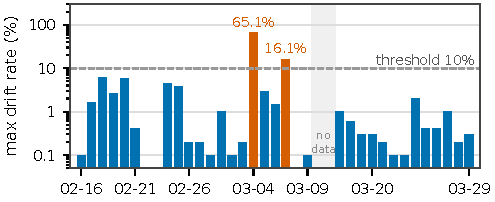
\includegraphics[width=\linewidth]{./figures/fig2-benchmark.pdf}
\caption{導入前ベンチマーク: 連続1日ペア35組の最大変動率(対数軸，破線はdb既定閾値10\%)．橙は実在の上流イベント(Red Hat VEX 65.1\%，SUSE OVAL 16.1\%)で，正常帯(中央値0.3\%)と桁で分離する．}
\label{fig:benchmark}
\end{figure}

\subsection{3つのチェック}
\label{sec:checks}

公開CIの圧縮後・公開前に，次の3チェックを実行する(検知結果差分の2つをDn(新スキャナ)とDo(旧スキャナ)，DB構造差分をDBと略記する)．

\begin{itemize}
\item \textbf{Dn: 検知結果差分(スキャナ最新版)}．
baselineとtargetの両DBに対して同一のスキャン結果fixture群(実機スキャン由来75ファイル，Windows系を含む12 OSファミリ+CPE系6ソース)でスキャナを実際に実行し，ファイル単位で検知CVE集合を比較する．fixture外の対象の検知退行はDBチェックのみが検出する．
変動率は(追加数+削除数)/baseline検知数で定義する．
\item \textbf{Do: 検知結果差分(固定した旧バージョンのスキャナ)}．
過去バージョンとの組でのみ現れる非互換退行(インシデント2型)を捕捉する．
\item \textbf{DB: DB構造差分}．
BoltDBを直接開き，ecosystem(後にソース単位へ細分化)ごとに検知条件木をleaf Criterionレベルまで平坦化して構造比較する．
スキャン結果もスキャナも不要でDBのみで完結する．
比較粒度をバイト列ではなくCriterionにしたのは，JSONキー順などの無害な変更での偽陽性を避けつつ，分母(全体で約330万Criterion)を大きく取り正常変動を小さなdriftとして吸収するためである．
\end{itemize}

各チェックは対象(ubuntu\_2204のようなfixtureファイル，またはubuntu:22.04のようなDB上のecosystemやソース)ごとの変動率を1\textbf{行}として出力し，1行でも閾値超過ならrunがFAILする(baseline不在の対象は100\%と扱う)．
チェック結果は変動率，増減の内訳，変動したCVEやアドバイザリのIDを含む構造化されたレポートとして常にCIのJob Summaryに出力される．
これは前稿が課題として挙げた「行ベース差分ではなく論理的な構造としての差分提示」\cite{nakaoka2025}の，公開品質管理という文脈での実装形でもある．
導入当初は最初のFAILで検査が停止する実装だったが，先にFAILしたチェックが後段のシグナルを隠す問題が判明し，現在は3チェックすべてを実行してから集約判定する．

\subsection{FAIL時の運用: 監査証跡付き手動promote}
\label{sec:promote}

候補DBは検査実行前にdigestのみ(タグなし)でGHCRにpushしておき，PASS時にのみタグを付けて「公開」する．
FAIL時は候補がタグなしのままdigestで取得可能に残り，事後検証できる．
オペレータがレポートを確認し正当な変更と判断した場合は，専用workflowで該当digestに手動でタグ付けする(promote)．
実行者，digest，タグがrun履歴に残り，「誰がどの候補をoverrideしたか」が追跡できる(判断対象のレポートはFAIL run側に残る)．
運用ルールとして，promoteの判断と実行は人間に限定している(AIエージェントには実行させない)．

\subsection{閾値のper-target / per-source化とgrooming}
\label{sec:threshold}

閾値はデフォルトでdetection 5\% / db 10\%とし，運用実績に基づき対象別に緩和するoverride機構を持つ(db 10\%は導入前ベンチマークに基づき，detection 5\%は経験的な初期値である)．
導入1ヶ月の運用で，新ディストリビューション立ち上がり期の一括triage，rolling release，ベンダ月次サイクルといった反復的な正当変動が毎回検査に引っかかることが判明したためである．
override値は失敗履歴の統計から「観測ピーク+ヘッドルーム」で導出し，単発スパイクはoverrideせずFAILさせて人間に見せる(例: EOLディストリビューションの39\%変動は異常として残置)．
リストの陳腐化を防ぐため約2ヶ月周期で全再導出する(grooming)．
さらに運用後期，ecosystem一括の変動率では大きなソースがノイズフロアになって小さなソースの異常を希釈する問題が顕在化し(\ref{sec:scaledist}節)，閾値もレポートもソース単位に細分化した．
なお変動率は追加と削除の対称量であり，overrideの緩和は検知漏れに直結する削除側の感度も同時に下げる．両方向を分けた非対称閾値は今後の課題である．

\section{測定方法論: 全数調査と原因帰属}
\label{sec:method}

\textbf{全数調査}:
本番導入(2026-04-23)から08-16までの116日間，2系統(安定版 / 開発版)の全943 runを対象に，runログ，PR，promote履歴をGitHub APIで全数収集した．
FAIL中はpromoteまでbaselineが動かず同じ差分で6時間おきに再FAILするため，run数は重複を含む．
そこで連続FAILを1つに潰したfail sequence(104件)，さらに2系統の統合とソース単位への分解を同時に行ったsource-episode(\textbf{69件})をイベントの正準単位として定義した．episodeは24時間以上の途切れで分割する集約規則であり，上流イベントの独立性の保証ではない(分割間隔を12h / 48hにすると77 / 62件になる)．episodeのソース族(targetが属するデータソースの系列)は全期間target名から推定し，後半窓ではレポートの明示ソースで内訳を検証した．

\textbf{原因帰属}:
各イベントについて，次の順で容疑を除外して原因を確定する．

\begin{enumerate}
\item \textbf{ビルダ除外}: baselineとtargetの両DBのメタデータに記録されたビルダのバージョンを比較する．一致すればDB構築コードは無罪．
\item \textbf{抽出器除外}: 対象期間の抽出器リポジトリのコミット履歴を走査する．当該ソースのfetch / extractコードに変更がなければ変換コードは無罪．
\item \textbf{取得設定除外}: 同期間のvuls-data-db(取得設定を持つリポジトリ)のコミットを走査する．取得対象のseedリストや新規データソースの追加がなければ取得設定は無罪．
\item \textbf{上流確定}: rawデータのGit履歴から対象期間のコミットを特定し，差分の中に変動と件数・IDが一致する変更実体(smoking gun．例えば新規アドバイザリファイル群やディレクトリの消失)を突き止める．
\end{enumerate}

この手順の各ステップは，履歴管理基盤\cite{nakaoka2025}の対応する工程の履歴にそれぞれ依拠している．
ビルダ除外はDBメタデータ，抽出器除外はコードのコミット履歴，上流確定はrawおよびextractedデータのGit履歴である．
全工程が履歴化されていなければ，例えば「上流の一時障害なので候補を破棄すべき」と「正当な変更なのでpromoteしてよい」の区別(\ref{sec:prevented}節)は当て推量になる．
逆に言えば，履歴管理は本測定の成立条件であり，前稿の基盤の実証でもある．
実際，全69 episodeをいずれかの工程に帰属し，「原因不明」は残らなかった．
ただし証拠の水準は一様ではない．
自前の処理由来と判定した10件のうち6件は原因のコミットやPRの差分を直接の証拠として特定したが，残る4件は開発版で先行したCPE関連変更系列への帰属であり，原因の工程までは確定していない．
上流由来と判定したepisodeは，ビルダ，抽出器，取得設定をコミット履歴の走査で除外した上での帰属であり，raw差分のsmoking gunまで確認したのは代表事例に限られる．
また帰属手順は再現可能なtriage手順書として整備し，AIエージェント用のスキルとしても記述している(役割分担は\ref{sec:guardrail}節)．

\textbf{妥当性への脅威}:
本稿の観測量は閾値を超えた事象に限られる打ち切り観測であり，閾値とoverrideという自分たちの設定に依存する．
したがって発動件数の絶対値ではなく，帰属の内訳と変動率の分布，および全変動を含む\ref{sec:benchmark}節のベンチマークを主たる根拠とする．
また検査自身も期間中に進化しており(3チェックの全実行化，fixtureとoverride追加，ソース単位化)，本データは固定測定器による同質標本ではなく進化する本番検査の発動履歴である．

\textbf{公開性}:
検査の実装(workflow，閾値，override設定)はvuls-data-db\cite{vuls-data-db}に，本調査のデータセット(run表からepisode別判定表まで)は公開リポジトリ\footnote{\url{https://github.com/vulsio/css2026-diff-guard}}にある．

\section{運用結果}
\label{sec:results}

\subsection{規模と原因分布}
\label{sec:scale}

943 run中，失敗は476 run．うち420 runが検査のステップで失敗した(閾値超過418+検査内インフラ障害2．残る56はビルド工程39とrunner障害等17)．
イベント単位では69 source-episodeである．
チェック別の捕捉はDB単独23件，Dn単独16件，複数同時30件，\textbf{Do単独0件}である(\ref{sec:blindspots}節)．
原因の分布を表\ref{tab:attribution}に示す．
内訳は上流由来59件，自前の処理由来10件である．自前由来のうち6件は原因のコミットやPRまで個別に特定し，残る4件は開発版で先行したCPE関連変更系列への帰属で工程は未確定である．

\begin{table}[tb]
\caption{episodeの代表判定の分布(計69件)．複数原因を含むepisodeは公開可否を左右した原因で代表させた．系列推定の4件は開発版で先行したCPE関連変更群への帰属で，工程(抽出器かビルダか)は未確定．他の自前由来6件は原因のコミットまで特定済み．上流由来(a)はfedora:46のような小規模baseline起因の構造的FAILを含む．捕捉列は発動したチェック．}
\label{tab:attribution}
\centering
\small
\setlength{\tabcolsep}{3pt}
\vspace{4pt}
\begin{tabular}{llll}
\hline
判定 & 件数 & 代表例 & 捕捉 \\
\hline
上流由来(a) 正当な変更 & 55 & 月次パッチ等 & 混在 \\
上流由来(b) 一時的障害 & 2 & CVRF消失 & Dn \\
上流由来(c) 恒久的品質イベント & 2 & errata再編 & 全て \\
抽出器由来(コードバグ) & 1 & 非決定的出力 & DB \\
抽出器由来(意図的変更) & 3 & 検知の補完 & DB \\
自前由来(系列，工程未確定) & 4 & 開発版cpe系列 & DB \\
取得設定由来 & 2 & seed追加 & DB \\
ビルダ由来 & 0 & (事例無し) & -- \\
\hline
\end{tabular}
\end{table}

観測期間の後半では，非上流由来のイベントが4件発生した．
2件は前半に存在しなかった\textbf{取得設定由来}である．
我々自身が取得対象のseedリストを拡張した直後(08-05〜06のWindows更新プログラム(KB) seed登録)にmicrosoft/microsoft-msucが211.3\%で発動し，新規データソースを追加した直後(08-10)にはmicrosoft/microsoft-servicingがbaseline不在のため100.0\%で発動した．
上流にも抽出器にも変更はなく「何を取りに行くか」の設定変更が原因で，vuls-data-db側のコミット走査(\ref{sec:method}節の手順3)を加えて初めて分離できた．
残る2件は\textbf{抽出器由来の意図的変更}の再来である．
代表例では，2012年から2022年の履歴的アドバイザリに検知を補完する抽出器変更(検知を持つファイルが643件から1,065件に増加)のマージ直後に，cpe\_fortinet/fortinet-cvrfが135.5\%で発動した．

\begin{figure*}[tb]
\centering
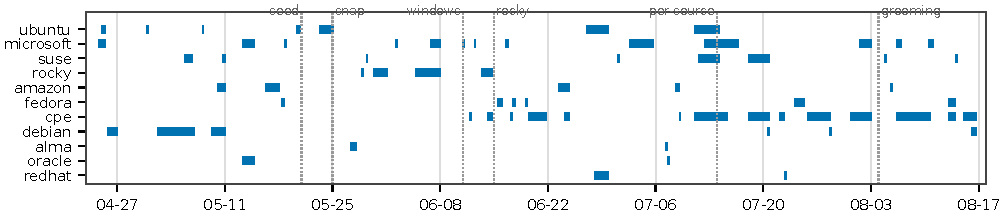
\includegraphics[width=\textwidth]{./figures/fig3-timeline.pdf}
\caption{116日間の発動タイムライン(source-episode 69件)．横棒は各episodeの持続期間(FAIL初出から終端まで)，点線は各override(seed，snap，windows，rocky，per-source化，grooming)の導入時点．per-source化後のcpe\_*系はcpe行に含めた．}
\label{fig:timeline}
\end{figure*}

\subsection{公開を阻止した3回}
\label{sec:prevented}

\begin{enumerate}
\item \textbf{Microsoft CVRF月次データ全消失(2回)}(CVRF: Common Vulnerability Reporting Framework):
上流APIが当月分のセキュリティ更新ドキュメント(700〜1,300ファイル)を丸ごと返さなくなり，Windows系13ターゲットで最大53.6\%の削除のみの差分が発生した(2回目は当月CVE約1,270件分の検知消失に相当)．
公開されていればインシデント1と同型の大量false negativeである．
検査は候補を破棄させ，上流回復後の再実行のみで復旧した．
raw履歴上，当月ファイル数は1273 $\rightarrow$ 0 $\rightarrow$ 1273 $\rightarrow$ 0 $\rightarrow$ 1278とフラッピングしており，単発の取得失敗ではなく上流配信自体の不安定であった．
\item \textbf{抽出器の非決定性バグ}:
rawの変更は266ファイルなのにextractedは23,163ファイル動くという異常をDBチェックが274.5\%のdriftとして検出した．
原因は抽出器が型の取り違えでソート処理をスキップし出力順序が非決定になっていたことで，修正PRに帰結した．
期間中唯一の「上流のせいではないコード起因の異常」の捕捉である．
\end{enumerate}

なお発動しないまま公開された破損は，利用者報告と事後の再分析の範囲では確認されていない(網羅的な検証手段は無い)．

\subsection{防ぎ切れなかった事例と検査改良の契機}
\label{sec:missed}

発動したが実害を防ぎ切れず，検査と運用の改良に帰結した事例が2件ある．

\begin{enumerate}
\item \textbf{AlmaLinux errataの縮退}:
errataフィードが1週間に複数回再編成され，アドバイザリ数が279から一時60まで減少，削除されたアドバイザリが参照していた434 CVEのうち87\%(376件)はフィード全体から消失し，残存アドバイザリでもkernel更新の検知条件が73から2パッケージへ縮退した(変動率は縮退時99.2\%，後述の巻き戻し時に最大428.3\%)．
過去バージョン系列に対する大量のfalse negativeに直結する．復旧作業でFAILの滞留を解消する際にオペレータが縮退候補をpromoteしてしまい，縮退DBは数時間公開に達したが，取り込みを縮退前のコミットにピン留めして同日中に巻き戻し，以後の流入を停止した．
その後，上流のHTML indexに残るのにフィードから消えたアドバイザリだけを取得履歴からfetch時に復元する機構を組み込みアンピンした．
ピン留めも復元も，取り込みの履歴管理が可能にする操作である(原因は\ref{sec:integrity}節)．
\item \textbf{VulnCheck一斉ロールアウト}:
単一コミットで145,672ファイル，+957万行という生成CPE(Common Platform Enumeration)設定の一斉付与をDBチェックが検出した．
ただし当時のecosystem一括の変動率では「cpe 28.9\%」としか言えず，候補はpromoteされた．
事後のソース単位の再分析で，当該ソース単独では189.6\%の変動であり，かつ実検知が60〜75\%消失する退行を含んでいたことが判明した．
この教訓がソース単位への細分化(\ref{sec:threshold}節)の直接の動機である．
「発動したが分解能不足で判定を誤りかけた」事例として記録する．
\end{enumerate}

2件とも検査は発動しており，止め切れなかったのは人間の承認判断である．残存リスクは検出側より承認側にあり，削除方向の自動ブロックや大規模消失時の複数名承認が次の改善点である．

\subsection{false positive論と運用ループ}
\label{sec:fp}

発動の大半は正当な上流変更であり，これを「誤報」と見るかは設計思想による．
本検査は安全ネットであり，822 CVEを単一アドバイザリに同梱するカーネル更新や，約600パッケージを束ねた単一アドバイザリ(5,312検知条件)のマス更新は，正当であっても公開前に人間が一目見るに値する．
一方，反復性が確立した既知の変動はoverrideで恒久緩和する．
116日間の手動promoteは92 unique digestに達し，この規模が\ref{sec:opscost}節の運用コストの実体である．

\section{考察: 観測された上流の危うさ}
\label{sec:discussion}

\subsection{消える・戻る・また消える(可用性)}
\label{sec:avail}

月次データの丸ごと消失(\ref{sec:prevented}節)は2ヶ月連続で発生し，2回目は2日間に消失と復活を4回繰り返した．
フィードの取得は「ある時点のスナップショット」であり，欠損の瞬間を取り込めばビルドは成功したまま欠損DBができあがる．
公開前の差分検査なしにこれを防ぐ手段は事実上ない．

\subsection{遡及的に書き換わる(完全性・一貫性)}
\label{sec:integrity}

\begin{itemize}
\item \textbf{errataの検知条件の縮退}:
AlmaLinuxのerrata縮退(\ref{sec:missed}節)では，フィード，OSV(Open Source Vulnerabilities)，HTMLの三者が一致したことから配信障害ではないと判断し，上流のissue trackerへ報告したところ，フィードが現行バージョンの情報しか保持しない仕様に起因するとの説明を得た\footnote{\url{https://bugs.almalinux.org/view.php?id=644}}．
上流が仕様どおりに動いていても，過去バージョンの範囲情報を必要とする脆弱性検知にとってはデータの欠損として働く例である．
\item \textbf{サイレントなサーバ側再編}:
Cisco openVuln APIでは，アドバイザリの更新日時もバージョンも一切変わらないまま，アドバイザリと影響バージョンのマッピングだけが日次で書き換わり，93アドバイザリから製品バージョン2,022件が削除された(例: 2014年のアドバイザリの製品リストが149から36へ)．
changelogにもissueにもアナウンスはない．
過剰マッピングの整理というデータ品質改善の側面が強い一方，該当バージョンを監視している利用者には黙った検知消失となる．
\item \textbf{一斉再生成の両義性}:
VulnCheckの全年代CVEへの生成CPE一括付与(\ref{sec:missed}節)は情報の拡充である一方，CPE語彙の現代化により既存のマッチングから外れる検知退行を同時に含んでいた．
2週間後，上流側の修正により退行の一部は「回復イベント」としてもう一度検査を発動させた．
拡充，退行，回復のいずれもが大変動として観測される．
\end{itemize}

\subsection{正当でも桁違いに動く(スケール)}
\label{sec:scaledist}

観測された最大変動率は3433.3\%(新規リリースfedora:46)，428.3\%(AlmaLinux errata再編)，305.9\%(CPE系)に達する一方，発動に至る日常変動は5〜20\%帯に収まり，両者は概ね桁で分離する．
ただし図\ref{fig:histogram}は閾値で打ち切られた分布である(\ref{sec:method}節の妥当性への脅威)．
ただし分離が崩れる構造要因が2つある．
(1) baselineが小さい対象は1バッチの正当な追加で容易に100\%を超える．
(2) FAILでbaselineが停滞すると比較窓が伸び，日常変動が蓄積して閾値を超える．
前者はper-target閾値，後者は迅速なpromote運用で吸収している．

\begin{figure}[tb]
\centering
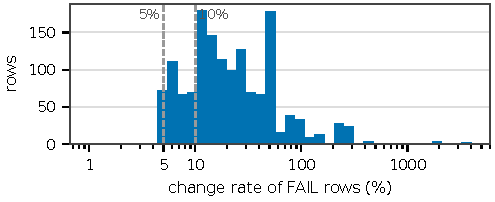
\includegraphics[width=\linewidth]{./figures/fig4-histogram.pdf}
\caption{全FAIL行(1,465行)の変動率分布(対数軸)．破線は既定閾値(detection 5\% / db 10\%)．閾値近傍の5〜20\%帯に対し，100\%超の構造イベント群が裾として分離する．FAIL行のみを重複(cron再実行)込みで集計した分布であり，全更新の変動率分布ではない．}
\label{fig:histogram}
\end{figure}

\subsection{チェックの相補性と検査の改良}
\label{sec:blindspots}

運用からは，チェック間の相補性と，検査自身の弱点の両方が見えた．
相補性の例がCVRF消失(\ref{sec:prevented}節の事例1)である．
DBチェックのKB比較はKBキーの集合しか見ないため，キー集合が不変のままCVEエントリが大量消失した本事例では0\%を返したが，観点の異なるDnが検知結果の激減として捕捉し公開を止めた．
単一の指標には盲点があり，それを補うのが多観点のチェックである(「KB 0\% $\neq$ 変化なし」は運用の警告事項として成文化した)．
一方，弱点として露呈し改良につながったものが2つある．
(1) ecosystem一括の変動率は大ソースが小ソースの異常を希釈した(ソース単位への細分化で対処)．
(2) overrideの系統間非対称が片系統だけの慢性FAILを生んだ(groomingで両系統を同時に見ることで対処)．
なお(1)のソース単位化の効果は後半の観測窓で実測できた．
レポートがソース名を持つため，前半では「cpe」と一括りだった変動が，vulncheck-nist-nvd2(110行)からjvn-feed-rss(5行)まで6ソースに分解された．
\ref{sec:missed}節のVulnCheck事例と同型の希釈は，後半の窓では観測されていない．

\subsection{運用コストの実態}
\label{sec:opscost}

検査は943 run中420(44.6\%)を止め，手動promoteは0.79件/日，ほぼ毎日1回人間がレポートを確認して承認している計算になる．
run単位のFAILの50\%は土日に発生しているが，これは上流ではなく人間側の信号である．
promoteが平日日中にしか行われないため，金曜夕方以降のイベントが週末じゅう再FAILし続ける(週末滞留)．
fail sequenceの持続時間(中央値11h / p90 48h)は検査の検出性能ではなくオペレータの応答時間の分布を測っており，通知や承認フローの自動化余地を見積もる直接の根拠となる．
また保留中は直前版が配られ続けるため，保留自体が新規CVEの反映遅延という別種のリスクを生む．
検査の実行時間はDBチェック約1分，検知チェック約9分で，6時間周期のCIに常設できる．

\subsection{開発プロセスに対する最終ガードレールとしての価値}
\label{sec:guardrail}

副次的だが実感の大きい価値として，パイプライン開発の最終防衛線がある．
テストやレビューが工程ごとのコードの正しさを検査するのに対し，データパイプラインの意味的な正しさは集約後の出力でしか観測できない．
実際，型の取り違えによるソート処理の欠落(\ref{sec:prevented}節)はコンパイルもテストも通過する類のバグであり，出力の構造差分としてのみ顕在化した．
また，開発版へ破壊的変更を先行投入して影響規模を定量観測する，予期したFAILの発現範囲が想定に閉じていることを混入なしの証拠に使う(\ref{sec:missed}節のピン解除)，といった能動的な使い方も定着した．
この「作られ方に依存せず生成物を検証する」性質は，AIエージェントがコード生成を担う開発形態で，コードレビューのスケール限界を補う出力レベルのガードレールとして重要性を増すと考える．本運用でも一次調査はAIエージェントに委ね，報告の検証とpromoteの判断は人間に限定している(\ref{sec:promote}節)．

\section{関連研究}
\label{sec:related}

\textbf{脆弱性データベースの品質}:
NVDをはじめとする脆弱性DBの品質は，影響バージョン不整合の検出\cite{dong19}，品質監査と自動修正\cite{anwar22}，国際比較\cite{lin26}，スキャナやSCA(Software Composition Analysis)ツール間の検知不一致のDB差への帰着\cite{imtiaz21,churakova25}，NVD enrichment停滞の定量化\cite{vulncheck24,anchore25}など，外部からの静的測定として繰り返し行われてきた．
本稿は測定器を本番の取り込み・公開パイプラインに常設し，フィードの経時変化を下流消費者の視点で縦断観測した点で異なる．

\textbf{セキュリティデータフィードの品質測定}:
脅威インテリジェンスフィードでは量，カバレッジ，遅延，正確性等の比較測定が行われ，フィード間の重複の少なさや品質の不可視性が示されている\cite{li19,bouwman20,griffioen20}．
いずれも外部からの横断測定であり，本稿は単一フィードを自身の公開履歴と比較する縦断測定を，公開を保留する運用機構として常設した点が新しい．

\textbf{データパイプラインの検証}:
宣言的制約によるデータ品質検証\cite{schelter18,breck19}や，パイプラインの実行履歴から検証基準を自動導出する研究\cite{tu23,redyuk21}がある．
本稿に最も近いのは，新しいデータバッチが履歴から逸脱した際に下流のML再学習をブロックするゲート\cite{shankar23}で，「履歴との比較で公開・利用を止める」という意味論まで本稿と同型である．
同ゲートが列統計の分布逸脱を信号としてMLの学習品質を保護するのに対し，本稿の検査は，(1)検知結果と検知条件構造という生成物の意味レベルの差分を信号とし，(2)セキュリティクリティカルな公開物を監査証跡付きのhuman-in-the-loop overrideで保護し，(3)さらに発動記録そのものを上流不安定性の測定データとして全数分析した，という3点で異なる．
本稿の検査は前公開版をオラクルとするdifferential testing\cite{mckeeman98}の時間軸変種，データへの回帰テスト\cite{yoo12}ともみなせる．

\textbf{国内の関連研究}:
国内では，脆弱性対策情報データベースJVNの提案\cite{terada05}以来の脆弱性情報流通の系譜に，OSSの脆弱性修正状況の調査\cite{kuzuno24}，PSIRT向けスクリーニング\cite{kanai24}などが続く．
IPAのJVN iPedia登録状況レポート\cite{ipa-jvnipedia}は2024年のNVD公開遅延が国内DBの登録数を減少させたことを記録しており，上流の不安定性が国内基盤へ波及する実例である．
フィード内容の経時的不安定性を定量計測した国内の学術研究は，我々の調査の範囲では見当たらない．

\section{おわりに}
\label{sec:conclusion}

脆弱性DBの公開CIに公開前検査を実装し，116日間・943 runの全数調査から69件の発動episodeを抽出して，59件を上流由来，10件を自前の処理由来に帰属した．
上流は消え，戻り，遡及的に書き換わり，アナウンスなく再編される．
しかもその大半は正当な変更である．
得られた知見は次の通りである．
(1)正常変動と異常イベントは変動率で概ね桁分離し，単純な閾値検査が実用になる．
ただし分解能(ソース単位)と閾値(対象単位のoverrideと定期grooming)は運用実績から継続的に導出する必要がある．
(2)発動原因の帰属は，収集・変換・構築の全工程が履歴管理されていることを成立条件とする．
前稿で報告した履歴管理基盤\cite{nakaoka2025}は，本測定と公開品質管理の土台として実証された．
本稿は同稿が課題として挙げた「差分の論理的な提示」「パイプラインの堅牢化」への，運用を伴う一つの回答でもある．
(3) FAIL時の復旧は「人間によるレポート確認+監査証跡付きoverride」として設計すべきである．誰がどの候補を通したかが履歴に残ることが，安全ネットを緩める操作の正当性を支える．
(4)上流の恒久的劣化には，取り込みのピン留めや自らの取得履歴からの復元という出口が要る．
(5)生成物を出力レベルで検証する検査は，自らの開発プロセスに対する最終防衛線としても機能し，テストとレビューをすり抜ける意味的バグの捕捉に実際に寄与した．コード生成にAIが入り込む開発形態でこの価値は増すと考える．

今後の課題として，fetch段階での欠損検出(月次ドキュメント丸ごと消失時にコミットしない等)，通知や承認フローの改善による週末滞留の解消，観測の長期蓄積による時系列特性の統計的確立，変動率の経過時間正規化による停滞バイアスの緩和，および同一上流を消費する他エコシステムとの観測の突合が挙げられる．

\bibliographystyle{junsrt}
\bibliography{./refs.bib}

\end{document}
